%----------------------------------------------------------------------------------------
%	PACKAGES AND OTHER DOCUMENT CONFIGURATIONS
%----------------------------------------------------------------------------------------

\documentclass[11pt]{scrartcl} % Font size

%----------------------------------------------------------------------------------------
%	PACKAGES AND OTHER DOCUMENT CONFIGURATIONS
%----------------------------------------------------------------------------------------

\usepackage{amsmath, amsfonts, amsthm} % Math packages

\usepackage{listings} % Code listings, with syntax highlighting

\usepackage[english]{babel} % English language hyphenation


\usepackage{booktabs} % Required for better horizontal rules in tables

\setlength\parindent{0pt} % Removes all indentation from paragraphs

\usepackage{enumitem} % Required for list customisation

\usepackage{graphicx} % Required for inserting images
\usepackage{tabularx} % For figures and tables

\usepackage[english]{babel} %set the language to English
\usepackage{lipsum}
\usepackage{caption}
\usepackage{float}
\usepackage{xstring}
\usepackage{pdfpages}
\usepackage{wrapfig}
\usepackage{hyperref}
\usepackage{longtable}
\usepackage{csquotes}


\usepackage{glossaries}

\graphicspath{ {./assets/} }

% for page numbering style
\renewcommand\thesection{\arabic{section}}

% Make glossaries
\makenoidxglossaries
\usepackage{pages/dict}

% Makes the text of glossary entries italic
\renewcommand{\glstextformat}[1]{\textit{#1}}

\setcounter{secnumdepth}{4}

%include this so that your paragraphs don't indent automatically
\setlength\parindent{0pt}

% No spacing between list items
\setlist{noitemsep}

\linespread{1.2}% line distance

% --------------- OPTIONAL ---------------------
\numberwithin{equation}{section} % Number equations within sections (i.e. 1.1, 1.2, 2.1, 2.2 instead of 1, 2, 3, 4)
\numberwithin{figure}{section} % Number figures within sections (i.e. 1.1, 1.2, 2.1, 2.2 instead of 1, 2, 3, 4)
\numberwithin{table}{section} % Number tables within sections (i.e. 1.1, 1.2, 2.1, 2.2 instead of 1, 2, 3, 4)
% ----------------------------------------------

%----------------------------------------------------------------------------------------
%	DOCUMENT MARGINS
%----------------------------------------------------------------------------------------

\usepackage{geometry} % Required for adjusting page dimensions and margins

\geometry{
	paper=a4paper, % Paper size, change to letterpaper for US letter size
	top=2.5cm, % Top margin
	bottom=3cm, % Bottom margin
	left=3cm, % Left margin
	right=3cm, % Right margin
	headheight=0.75cm, % Header height
	footskip=1.5cm, % Space from the bottom margin to the baseline of the footer
	headsep=0.75cm, % Space from the top margin to the baseline of the header
	%showframe, % Uncomment to show how the type block is set on the page
}

%----------------------------------------------------------------------------------------
%	FONTS
%----------------------------------------------------------------------------------------

\usepackage[utf8]{inputenc} % Required for inputting international characters
\usepackage[T1]{fontenc} % Use 8-bit encoding

\usepackage{fourier} % Use the Adobe Utopia font for the document

%----------------------------------------------------------------------------------------
%	SECTION TITLES
%----------------------------------------------------------------------------------------

\usepackage{sectsty} % Allows customising section commands

\sectionfont{\vspace{6pt}\centering\normalfont\scshape} % \section{} styling
\subsectionfont{\normalfont\bfseries} % \subsection{} styling
\subsubsectionfont{\normalfont\itshape} % \subsubsection{} styling
\paragraphfont{\normalfont\scshape} % \paragraph{} styling

%----------------------------------------------------------------------------------------
%	HEADERS AND FOOTERS
%----------------------------------------------------------------------------------------

\usepackage{scrlayer-scrpage} % Required for customising headers and footers

\ohead*{} % Right header
\ihead*{} % Left header
\chead*{} % Centre header

\ofoot*{} % Right footer
\ifoot*{} % Left footer
\cfoot*{\pagemark} % Centre footer

%----------------------------------------------------------------------------------------
%	CITING STUFF
%----------------------------------------------------------------------------------------
%use this exact command. The style and bibliographystyle has to be author year (Harvard). The sorting is nyt: name, year, title so that the bibliography is sorted alphabetically. firstInits=true shortens the names: Albert Einstein -> A. Einstein
\usepackage[backend=bibtex,style=authoryear,bibstyle=authoryear,sorting=nyt,firstinits=true,uniquename=init]{biblatex}
% Declare custom cite command for personal communication (optional)
\DeclareAutoCiteCommand{inline}{\mycite}{\cites}
\DeclareCiteCommand{\mycite}
 {}{\ifentrytype{misc}{%
 \IfStrEq{\thefield{howpublished}}{personal communication}
 {\mkbibparens{\printnames{labelname}, personal communication, \printdate}}
 {\mkbibparens{\usebibmacro{cite}}}%
 }
 {\mkbibparens{\usebibmacro{cite}}}%
 }{}{}
% End of custom cite command % Include the file specifying the document structure and custom commands

\usepackage{glossaries}
% Make glossaries
\makenoidxglossaries

% Makes the text of glossary entries italic
\renewcommand{\glstextformat}[1]{\textit{#1}}

% Glossary entries
\newglossaryentry{ExtJs}
{
    name=ExtJs,
    description={ExtJS is a JavaScript framework for building web applications with a rich user interface}
}

\newglossaryentry{Hadoop}
{
    name=Hadoop,
    description={Hadoop is a distributed processing framework written in Java that allows for large-scale data storage and processing}
}

\newglossaryentry{Nodejs}
{
    name=Nodejs,
    description={Node.js is an open-source, cross-platform JavaScript runtime environment that enables server-side scripting}
}

\newglossaryentry{Expressjs}
{
    name=Expressjs,
    description={Express.js is a lightweight and flexible web application framework for Node.js used for building scalable and efficient server-side applications~\parencite{expressjs}}
}

\newglossaryentry{Postgresql}
{
    name=Postgresql,
    description={PostgreSQL is a powerful, open-source object-relational database system that provides advanced features for scalability, reliability, and data integrity}
}

\newglossaryentry{Reactjs}
{
    name=Reactjs,
    description={React.js is a JavaScript library that allows the creation of interactive user interfaces using reusable UI components}
}

\newglossaryentry{ReCharts}
{
    name=ReCharts,
    description={ReCharts is a lightweight, open-source, charting library that provides a wide range of customizable charts and graphs for data visualization}
}

\newglossaryentry{Weather API}
{
    name=Weather API,
    description={Weather API is an API provided by weatherapi.com that provides real-time weather data for a wide range of locations and parameters}
}

\newglossaryentry{Python}
{
    name=Python,
    description={Python is a high-level, interpreted programming language with dynamic semantics that is widely used in various fields, including data science, machine learning, and web development}
}

\newglossaryentry{Tensorflow}
{
    name=Tensorflow,
    description={TensorFlow is an open-source machine learning framework developed by Google for building and training neural networks}
}

% Acronyms
% \newacronym{cms}{CMS}{Conten Management System}

 % Include the file specifying the glossary / acronym entries

\addbibresource{main.bib}

%----------------------------------------------------------------------------------------
%	TITLE SECTION
%----------------------------------------------------------------------------------------

\title{	
	\normalfont\normalsize
	\textsc{Fontys University of Applied Sciences \\A research conducted for the minor A-Systems}\\ % Your university, school and/or department name(s)
	\vspace{25pt} % Whitespace
	\rule{\linewidth}{0.5pt}\\ % Thin top horizontal rule
	\vspace{20pt} % Whitespace
	{\huge IoT soil moisture monitoring to predict irrigation needs of outdoor crops}\\ % The assignment title
	\vspace{12pt} % Whitespace
	\rule{\linewidth}{2pt}\\ % Thick bottom horizontal rule
	\vspace{12pt} % Whitespace
}

\author{\LARGE Niklas Mezynski} % Your name

\date{\normalsize\today} % Today's date (\today) or a custom date

\begin{document}

\maketitle % Print the title

% Remove page number from title page
\thispagestyle{empty}

\newpage


%----------------------------------------------------------------------------------------
%	ToC and page/section numbering
%----------------------------------------------------------------------------------------

\pagenumbering{roman}

% Table of contents depth of contents
\setcounter{tocdepth}{3}
\tableofcontents

\newpage
\listoffigures

\newpage
\listoftables

\clearpage
\printnoidxglossaries
\cleardoublepage
\pagenumbering{arabic}
\setcounter{section}{1}

%----------------------------------------------------------------------------------------
%	BEGIN CONTENT
%----------------------------------------------------------------------------------------

\subsection{Introduction}
\subsubsection{Background and context}
Soil moisture monitoring is a crucial aspect of modern agriculture. The accurate monitoring of soil moisture levels can improve crop yields, save water, and increase efficiency. Currently, many farmers use manual methods to monitor soil moisture levels, which can be time-consuming and imprecise. In recent years, IoT sensors have been developed, which can provide real-time data on soil moisture levels~\parencite{bwambale2022smart}.
\newline Although there are various sensors already being used in modern agriculture, it is not clear which sensor is the most accurate and effective for different soil types, crop types, and environmental conditions. Additionally, the integration of weather data in irrigation scheduling is often not being considered~\parencite{nandurkar2014design}.
\newline Moreover, the traditional manual methods of monitoring soil moisture levels and irrigation scheduling are labor-intensive, time-consuming, and often based on assumptions rather than actual data. This results in excessive water usage, which not only wastes a valuable resource but also impacts the environment negatively~\parencite{bwambale2022smart}.
\newline Therefore, the lack of an accurate and efficient system for monitoring soil moisture levels and predicting crop irrigation needs results in a significant gap in knowledge in the agricultural industry. Through this research project, the aim is to develop a cloud-based application that can accurately monitor soil moisture levels, integrate weather data, and predict crop irrigation needs.

\subsubsection{Research questions and objectives}
This study's research question seeks to investigate the efficacy of a cloud-based application that integrates real-time soil moisture and weather data in predicting the irrigation needs of outdoor crops, as well as how it compares to traditional manual irrigation scheduling methods. The study has identified several theoretical learning objectives to accomplish this.
\newline Understanding the principles of IoT sensors and their applications in agriculture, the basics of cloud computing and monitoring and their applications in agriculture, exploring algorithms for predicting crop irrigation needs using soil moisture and weather data, finding a correlation between certain weather data parameters and changes in soil moisture levels to make predictions, and developing a cloud-based monitoring application that can make a decision are some of the objectives. The study's goal is to shed light on the efficacy of cloud-based applications and how they may be utilized to enhance crop irrigation, ultimately contributing to the development of sustainable and efficient agricultural practices.
\subsubsection{Overview of the experiment and methods}
The experiment will take place in an open field-like setting. The experiment will be divided into two phases. In the first phase, soil moisture levels will be monitored and data is collected using IoT sensors. In the second phase, the collected data will be used to develop a cloud-based application that can predict irrigation needs for outdoor crops. The experiment will take place over the course of four weeks. The first two weeks will be spent collecting data, and the following two weeks will be spent verifying the algorithm and its efficiency. The experiment will be carried out as follows:
\begin{itemize}
	\item The soil moisture levels will be monitored using IoT sensors.
	\item The data will be collected and stored in a database.
	\item The data will be analyzed to find a correlation between certain weather data parameters and change in soil moisture levels.
	\item The data will be used to develop a cloud-based application that can predict irrigation needs of outdoor crops.
	\item The algorithm will be verified and its efficiency will be tested.
\end{itemize}

\subsection{Literature review}
\subsubsection{IoT sensors and their applications in agriculture}
Agriculture is facing huge challenges as a result of population growth and climate change. It is critical to establish sustainable techniques in order to meet the demands for food production. IoT sensors, for example, have the potential to change agriculture and address these difficulties. The use of IoT sensors and wireless sensor networks into agriculture has created new prospects for precision farming and resource optimization.~\parencite{capacitive_sensors_for_irrigation_and_disease}
\newline A smart irrigation system was presented in one study that used IoT and machine learning to offer correct irrigation to plants. The technology lowered water consumption by 46\% while enhancing plant health. Another study built a low-power and scalable IoT-based architecture to monitor soil moisture and temperature for home farmers and scientific applications. The measured data was sent to a cloud platform for processing, providing home farmers with critical information to improve crop efficiency and reduce crop failure. The study's hardware and software architecture were designed to require less power, making it an efficient and cost-effective solution.~\parencites{precision_irrigation_iot}{capacitive_sensors_for_irrigation_and_disease}
\newline The application of IoT sensors in agriculture has also demonstrated promise in smart farming and precision agriculture. Sensors can be used to detect illnesses, test NPK levels, and detect soil moisture content, among other things. Smart farming optimizes traditional farming processes by utilizing precise information to make informed decisions. Control and supervision, safety, warning, diagnostics, and analytics are all applications of IoT sensors in agriculture, making it more effective and trouble-free.~\parencite{iot_and_sensors_in_agriculture_general}
\newline Finally, IoT sensors provide several benefits to agriculture, including reduced water usage, increased efficiency, fewer crop failures, and improved yield. As the world population expands and food demand rises, the use of IoT and sensor networks in agriculture will become even more vital in order to provide food for everyone in a sustainable manner.\parencite{capacitive_sensors_for_irrigation_and_disease,bwambale2022smart}
\newline There could be numerous reasons for the low number of real-world uses of soil moisture sensors in open fields. One issue is the high cost and complexity of sensor installation and maintenance, which can be too expensive for many farmers. Furthermore, there may be a lack of understanding and education regarding the benefits of employing soil moisture sensors, as well as the best practices for using them. Finally, regulatory and policy constraints may exist that limit the deployment of certain technologies in specific regions or countries. More study is required to overcome these issues and promote the wider use of IoT sensors for sustainable agriculture practices.

\subsubsection{Cloud computing and monitoring in agriculture}
A 2019 study explores the development of a networking application system for modern agriculture with the goal of addressing agricultural product quality safety and environmental contamination. Their solution is built on open-source hardware, which makes video surveillance based on motion detection easier. In the development and implementation of a demo system, the authors created a basic cloud platform system for modern farm network monitoring that employs a RESTful interface service system and \gls{ExtJs} client technology. The \gls{Hadoop} platform is utilized to achieve huge data processing generated by Internet of Things applications, and the associated model is developed using machine learning technology. The research addresses crop variety selection, production and cultivation management, and time to market.~\parencite{cloud_computing_and_monitoring}
\newline Currently, Internet of Things-related technologies and products are becoming more mature, and the associated software and hardware facilities, technical standards, and transmission protocols are being gradually upgraded. These mature hardware and software solutions are used in agricultural production for data collection, transmission, storage, processing, feedback, and control.~\parencite{cloud_computing_and_monitoring}
\newline The study focuses on the advantages of cloud computing in the Internet of Things. The cloud platform provides an easy sensing data transmission interface for the sensing device, and the user can easily transmit data acquired by the sensor to the cloud platform. The cloud platform stores, analyzes, and processes data, as well as providing informative feedback based on user-defined decision rules. Users can also use the platform for equipment administration, data inquiry, visualization, warning, information push, and other operations via a web interface or mobile app. The cloud services platform improves the security, stability, and low-cost operation of the necessary applications, allowing developers to focus on application development.~\parencite{cloud_computing_and_monitoring}
\subsubsection{Biological Aspects of Soil Moisture and Crop Irrigation Needs}
\paragraph{The effect of soil moisture on plant growth and yield}
Soil moisture is an important aspect of plant growth and development. The relationship between soil moisture and crop development, yield, and quality is detailed in this section. Also covered is the significance of available moisture for irrigation control, nutrient uptake, and drought management.~\parencite{soil_moisture_plant_water}
\newline Soil moisture is influenced by a variety of factors, including soil type, climate, rainfall, irrigation, and soil management practices. The texture, structure, and organic matter composition of the soil determine its water-holding ability. Understanding these elements is critical for good soil moisture management.~\parencite{soil_moisture_plant_water}
\newline The maximum amount of water that soil can hold after surplus water has been drained away and the rate of downward flow has been reduced is referred to as field capacity. When the soil is at \textbf{field capacity}, it can hold the maximum quantity of water available to plants without becoming waterlogged or generating anaerobic conditions. The soil moisture content at which plants can no longer take water from the soil, causing wilting and eventually death if the water supply is not restored, is known as the \textbf{permanent wilting point}.~\parencite{soil_moisture_plant_water}
\newline Soil moisture has an impact on several aspects of agriculture. One being the impact on crop growth and yield. Adequate soil moisture is necessary for optimal crop growth and development, which directly impacts crop yield and quality. Insufficient soil moisture can lead to plant stress, reduced growth, and lower yields, while excessive soil moisture can cause waterlogging, root rot, and other issues.~\parencite{soil_moisture_plant_water}
\newline Knowing the available moisture in the soil also allows for more efficient irrigation scheduling and water management. By ensuring that the soil moisture stays within the range between field capacity and the permanent wilting point, farmers can optimize water use, prevent over- or under-watering, and promote healthy plant growth.~\parencite{soil_moisture_plant_water}
\newline Soil moisture is also important for the availability and uptake of nutrients by plants. Many nutrients dissolve in soil water and are absorbed by plant roots via the water uptake process. Farmers can ensure that plants have access to vital nutrients for growth and development by maintaining appropriate soil moisture levels.~\parencite{soil_moisture_plant_water}
\newline In conclusion, soil moisture is an important factor in crop growth, yield, and quality. Farmers must effectively manage soil moisture in order to maximize crop production and ensure sustainable agriculture.
% \subsubsection{Physiological responses of plants to water stress}
% \subsubsection{Advantages and disadvantages of using soil moisture as an indicator for crop irrigation needs}


\subsection{Experiment}
\subsubsection{Design and setup}
The first stage of the experiment is dedicated to data collection. For the experiment, a few salad crops are planted in a pot that is set outside in the open air to allow rain, sun, and other weather factors to fully affect them. In addition, a soil moisture sensor (Section~\ref{sec:sensors}) linked to an ESP32 is embedded in the soil. The setup can be seen in Figure~\ref{fig:experiment_setup}.
\begin{figure}[h]
	\centering
	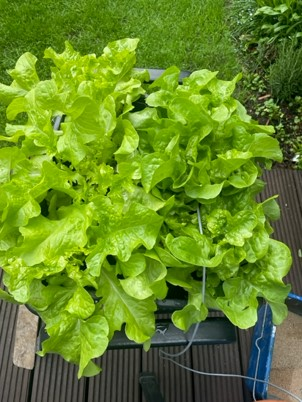
\includegraphics[height=5cm]{setup.jpg}
	\caption{Experiment setup}
	\label{fig:experiment_setup}
\end{figure}
The data is gathered from the soil moisture sensor and wirelessly transmitted to a web server, where it is kept in a database with current meteorological data obtained from an API. The information gathered will subsequently be utilized to train a machine learning model that will forecast the crop's irrigation requirements. Section~\ref{sec:data_collection} explains how the data is visualized on a web page.

\paragraph{Sensors}
\label{sec:sensors}
% TODO: Still needs sources
Capacitive soil moisture sensors are a common type of sensor for measuring soil moisture levels. Capacitive sensors, as opposed to other sensors that measure moisture based on resistance, rely on the electrical capacitance of the soil, which changes with soil moisture content, allowing the sensor to measure the soil moisture level.~\parencite{sensor_types}
\newline The accuracy of capacitive soil moisture sensors is one of their key advantages. They are quite precise, even in soils with variable compositions. They are also reasonably inexpensive and simple to install, making them a viable option for sensing soil moisture in wide regions. Furthermore, they are unaffected by the presence of salts or other substances in the soil, which might impair the accuracy of other types of sensors.~\parencite{sensor_types}
\newline For these reasons, using capacitive soil moisture sensors to measure crop water needs is a good option, especially when accurate data is required in a lab setting. They provide a more accurate and consistent measurement of soil moisture levels, which is essential for effective irrigation control. Several sensors will still be used to account for the spatiotemporal variability of field-scale soil moisture.~\parencite{sensor_types}
\subsubsection{Data collection and analysis}
\label{sec:data_collection}
In order to retrieve and store the sensor data, a cloud based system was developed using \gls{Nodejs}. It uses \gls{Expressjs} under the hood to expose RESTful API endpoints the ESP32 can use to send the data. The data is then stored in a \gls{Postgresql} database. The data is then visualized on a web page using \gls{Reactjs} and \gls{ReCharts}. The web page can be seen in Figure~\ref{fig:web_page}.
Each time a new sensor value is received, the backend will also query the current weather data from the \gls{Weather API} API. This data is also stored in the database.
\begin{figure}[h]
	\centering
	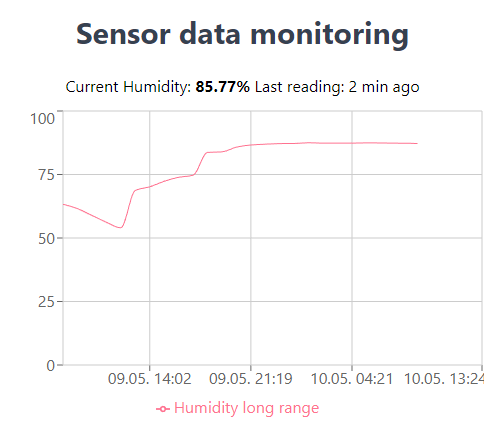
\includegraphics[width=6cm]{web_page.png}
	\caption{Web page}
	\label{fig:web_page}
\end{figure}
\newline After enough data is collected, it is going to be analyzed using \gls{Python} and \gls{Tensorflow} to train a machine learning model that will forecast the crop's irrigation requirements.

\subsection{Results}
\subsubsection{Overview of the collected data}
The data collected from the sensors and the weather API is shown in Figure~\ref{fig:collected_data}. The data was collected over a period of 3 weeks. The values that have been tracked were the soil moisture, the temperature, the humidity, the UV-Index, the cloud coverage, the pressure, and the precipitation.
\begin{figure}[h]
	\centering
	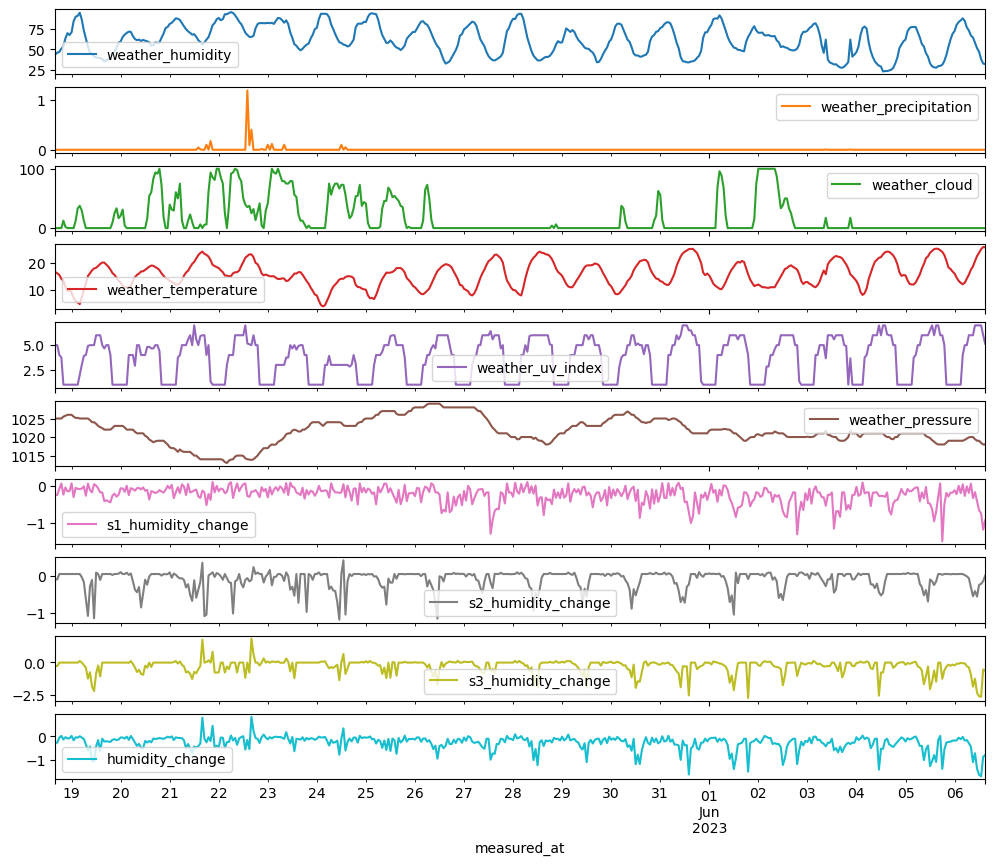
\includegraphics[width=\textwidth]{collected_data.png}
	\caption{Collected data}
	\label{fig:collected_data}
\end{figure}

\subsubsection{Correlation analysis between weather data and soil moisture}
In order to determine the correlation between the weather data and the soil moisture, a correlation matrix was created. The correlation matrix can be seen in Figure~\ref{fig:correlation_matrix}. The correlation matrix shows that the soil moisture is highly correlated with the temperature and the humidity. The soil moisture is also slightly correlated with the UV-Index and the cloud coverage. The soil moisture is not correlated with the pressure.
\begin{figure}[h]
	\centering
	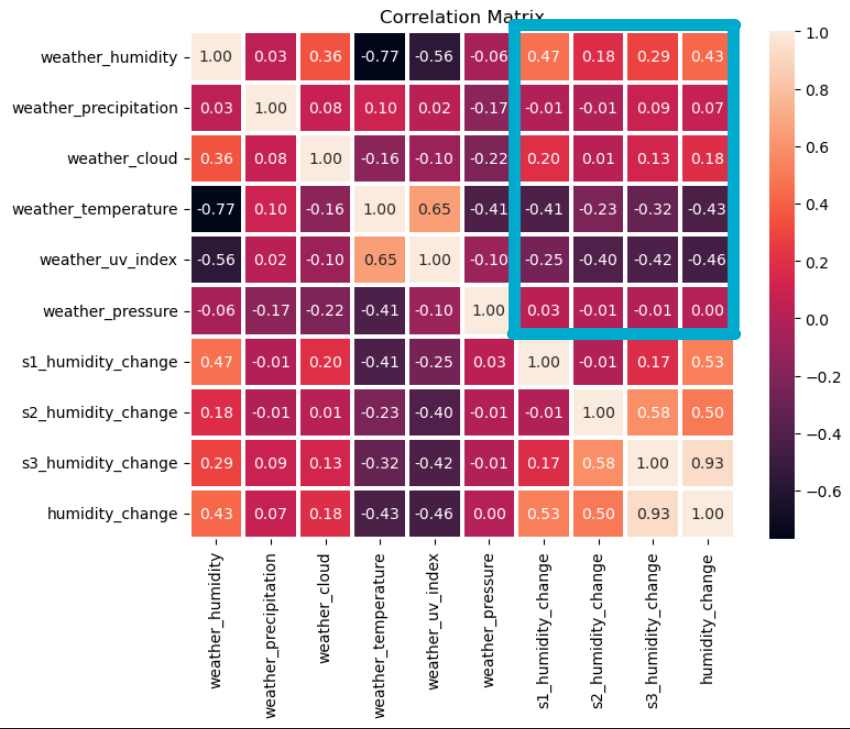
\includegraphics[height=9cm]{correlation_matrix.png}
	\caption{Correlation matrix}
	\label{fig:correlation_matrix}
\end{figure}
\newline Considering the four most significant factors:
\begin{equation*}
	\begin{aligned}
		Weather\ precipitation\ (mm)              & := w_p \\
		Weather\ temperature\ (^{\circ} C)        & := w_t \\
		Weather\ humidity\ (\%)                   & := w_h \\
		Weather\ UV-Index                         & := w_u \\
		Soil\ moisture\ change\ (\frac{\%}{hour}) & := s_m \\
	\end{aligned}
\end{equation*}
\newline The following linear regression model can be created:
\begin{equation*}
	\begin{aligned}
		\Rightarrow s_m = 0.503375w_p -0.013527w_t + 0.002103w_h -0.042218w_u -0.041001
	\end{aligned}
\end{equation*}

\subsubsection{Comparison between cloud-based irrigation scheduling and traditional manual methods}
TODO: Still has to be evaluated. The experiment is still running.
\subsection{Discussion}
\subsubsection{Implications of the results for precision agriculture and water management}
TODO: Still has to be evaluated. The experiment is still running.

\subsubsection{Limitations of the experiment and possible improvements}
\label{sec:limitations}
There are several limitations to this experiment. The first limitation is that the experiment was conducted on a small scale. Only six salad plants were used in total, and they do not consume much water at all. The second limitation is that the experiment was conducted over a short period of time. The plants were only watered for three weeks. The third limitation is that the experiment was conducted in a controlled environment. The plants were watered with a fixed amount of water every day. In a real-world scenario, the plants would be watered with a variable amount of water every day.
\newline There are also several limitations to the regression model. One being that the experiment was conducted with a single type of plant. The results might be different for other types of plants. Also, factors like soil type and quality, growth stage, and the plant's health were not taken into account.

\subsubsection{Future directions for research}
This section will cover what needs to be done in order to eliminate the limitations listed in section \ref{sec:limitations}.

\subsection{Conclusion}
\subsubsection{Summary of the research questions and objectives}
The goal of this study was to find out if it is possible to use cloud computing and regression algorithms to predict the irrigation needs of a crop. The study also aimed to find out if it is possible to use a cloud-based system to collect and analyze the data.

\subsubsection{Contributions of the study to the field}
This study does only offer a proof of concept. It shows that it is possible to use cloud computing and regression algorithms to predict the irrigation needs of a crop. The study also shows that it is possible to use a cloud-based system to collect and analyze the data.
\newline Although this technique does not deliver perfect results, it is a very cheap and (for the farmer) easy to implement method. The costs of the sensors are relatively low, and the data can be collected and analyzed in the cloud. The farmer does not have to do anything except for installing the sensors and connecting them to the internet. In a well implemented system the farmer does not have to worry about the data collection and analysis. An automated calibration phase could be enough to make precise predictions. Also, the model could be improved by further enhance the regression model based on the data it collects while it is running.
\newline The sensors could be connected through a LoRa network to monitor the soil moisture of a whole field. The sensors could be connected to a LoRa gateway, which would then send the data to the cloud.
\newline The whole thing could possibly be sold as a service. The farmer would only have to pay a monthly fee for the service. The service provider would then take care of supplying and calibrating the right sensors. The provider would also take care of the data collection and analysis. The farmer would only have to install the sensors and connect them to the internet.
\subsection{Final remarks and recommendations}


\newpage
\printbibliography[title=References]
\end{document}


